\documentclass[twocolumn,conference]{IEEEtran}
\usepackage[pdftex]{graphicx}
\usepackage{fullpage,graphicx,psfrag,url,caption}
\usepackage{amsmath,amsfonts,amssymb}
% \topmargin=-0.5in
% \textheight=9in
% \oddsidemargin 0in
% \evensidemargin 0in
%5\textwidth 6.5in
\usepackage{indentfirst}
% \setlength{\parindent}{2em}
\usepackage{fancyhdr}
\pagestyle{fancy}
\fancyfoot[l]{EE122, Spring 2019}
\fancyfoot[r]{Introduction to communicatino networks}  %%% change C to L or R as needed
\renewcommand{\headrulewidth}{0pt}
\renewcommand{\footrulewidth}{0pt}
\usepackage[colorlinks,linkcolor=red,anchorcolor=blue,citecolor=green]{hyperref} 

% \fancypagestyle{plain}{
%    % \fancyhf{Conference}
%    % \fancyhead[C]{Conference on \LaTeX}   %% C or L or R.
%    % \fancyfoot[L]{This is a notice}%            %% C or L or R.
%    \renewcommand{\footrulewidth}{0pt} 
%    \renewcommand{\headrulewidth}{0pt}
% }
% \usepackage{fancyhdr}
% \pagestyle{fancy}
% \lhead{EE122, Spring 2019}
% \rhead{Introduction to communicatino networks}
% \renewcommand{\headrulewidth}{0.4pt}
\renewcommand{\footrulewidth}{0.4pt}

\begin{document}
\title{\textbf{Simulation about the difference between 
FDM system and OFDM system
}}
\author{Caiqian Cheng, Yuechen Wu, Hang Zhou
}
\maketitle
% \markboth{Journal of Quantum Telecommunications, ̃Vol . ̃1, No. ̃1, ̃January ̃2025}{Shell \MakeLowercase{\text it{et al.}}: A Novel Tin Can Link}
\thispagestyle{fancy}
\begin{abstract}
This paper presents the analysis of the comparison between FDM system vs OFDM system. Three comparison method is implemented, mathematically, software simulation and hardware simulation.
\end{abstract}



\section{Introduction}
Just to clarify, in the progress report and the abstract, our group is comparing the single carrier system with the OFDM, but now we change to the comparison between FDM and OFDM. The reason is because that if using single carrier, the throughput of single carrier will be incredibly low compared to OFDM. So in order to compare when the throughput is similar, we change the topic to be ‘The comparison between FDM and OFDM.

This project is about the comparison between FDM (Frequency Division Multiplex) and OFDM (orthogonal frequency-division multiplexing). We implemented the comparison through three aspects, theoretically, software simulation and hardware simulation.



\section{Theory}
To prove that OFDM is better than FDM in theory, we learnt a lot about the techniques they are using.


Here's the comparision between the FDM and OFDM
\subsection{Orthogonal Derivation}
    \begin{itemize}
        \item Discrete set of N carriers over a symbol interval of finite length T
        \[
        u(t)=\sum_{n=0}^{N-1}B[n]e^{j2\pi f_nt}I_{[0,T]}(t)=\sum_{n=0}^{N-1}B[n]p_n(t)
        \]

        \item The symbols B[n] are mapped to the carriers.
        \[
        u(t)=\sum_{n=0}^{N-1}B[n]e^{j2\pi f_nt}I_{[0,T]}(t)=\sum_{n=0}^{N-1}B[n]p_n(t)
        \]

        \item Orthogonality for two sub-carriers $p_n(t)$ and $p_m(t)$:
        % \begin{equation}
        % \begin{split}
        % <p_n,p_m>&=\int_{0}^{T}e^{j2\pi f_nt}e^{-j2\pi f_mt}dt\\
        % &=\frac{e^j2\pi(f_n-f_m)T-1}{j2\pi(f_n-f_m)}
        % \end{split}
        % \end{equation}
        \[\begin{aligned}
            <p_n,p_m>&=\int_{0}^{T}e^{j2\pi f_nt}e^{-j2\pi f_mt}dt\\
        &=\frac{e^j2\pi(f_n-f_m)T-1}{j2\pi(f_n-f_m)}
           \end{aligned}\]
        orthogonal if $(fn-fm)T$ is non-zero integer; for example $f_n = \frac{n}{T}$

        \item Fourier transform of $p_n(t)$:
        \[
        P_n(f)=T\cdot sinc((f-f_n)T)e^{-j\pi(f-f_n)T}
        \]

        

    \end{itemize}

\subsection{Comparision}
    \subsubsection{Band Number}\hfill\\
    \indent Compared by the number of bands we need, FDM is using independent single carriers to transmit the signal while OFDM is using orthogonal sub-carriers inside one carrier to transmit. The fact that FDM is using independent single carriers means that if N users want to send information at the same time, N users will be assigned to N bands ( single carriers ). The more the people is, the more bands it needs. While for OFDM, one band is divided into smaller sub-bands. If one band has M sub-bands, all the band number we need will be around $\frac{N}{M}$. Although this example is too simple and doesn’t take into account the baud rate (which we will discuss later), we still get a taste of how OFDM can save more ‘space’ in frequency domain.
    
    \hfill\\\subsubsection{Frequency Utilization}\hfill\\
    \indent Compared by the frequency utilization, the FDM is using guard band while OFDM doesn’t need guard band. For FDM, to prevent aliasing between bands, it insert a ‘empty band’ between all the bands so that information don’t get overlapped. Frequency bands,  being non Renewable resources, should be assigned properly. For OFDM, it doesn’t use guard band, so its frequency efficiency can be higher.
    \begin{figure}[h]
        \centering
        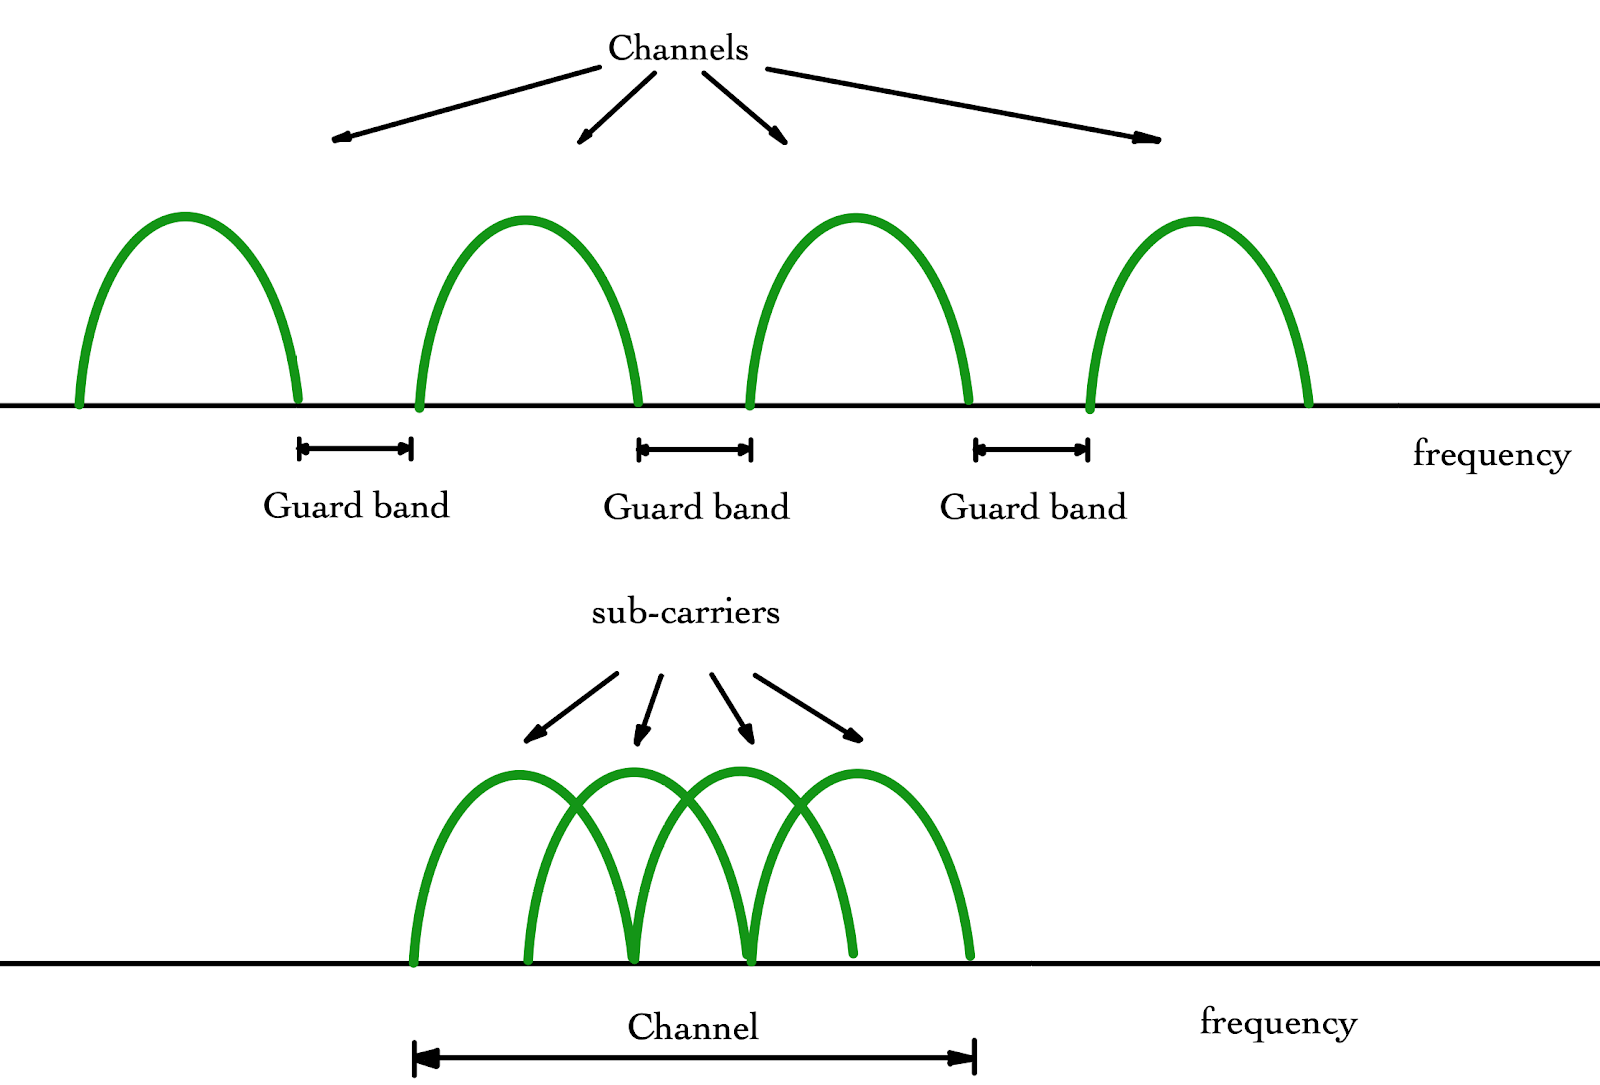
\includegraphics[width=0.5\textwidth]{./asset/freq}
        \caption{frequency utilization}
        \label{fig:frequency utilization}
    \end{figure}

    \hfill\\\subsubsection{Temporal Utilization}\hfill\\
    \indent Compared by the temporal utilization, the OFDM has a technique called time division. Not only the frequency domain is divided into different sub-bands, the time domain is also divided into different time slots. Under this circumstances, the assignment of the time and frequency is more flexible.

    \hfill\\\subsubsection{Inter Symbol Interference}\hfill\\
    \indent Compared by the ISI ( Inter Symbol Interference ), the OFDM will be much more robust compared to FDM. For FDM, each symbol is transmitted on one channel. If part of the channel is distorted, the whole message sending in the channel will the lost. For OFDM, each symbol is transmitted on one sub-channel. If part of the channel is distorted, some of the message will still get distorted and lost, but most of them can still be perfectly received at the receiver end.
    \begin{figure}[h]
        \centering
        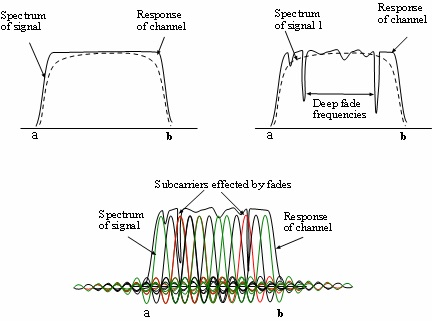
\includegraphics[width=0.5\textwidth]{./asset/ISI}
        \caption{Inter Symbol Interference}
        \label{fig:Inter Symbol Interference}
    \end{figure}

    \hfill\\\subsubsection{Multi Path Fading}\hfill\\
    \indent Compared by the multi path fading effect, the OFDM uses cyclic prefix to avoid this effect while FDM doesn’t. For OFDM, each symbol’s tail part is copied and added at the front. In this case, each symbol is a little longer. The copied version of the tail at the front is called cyclic prefix. The length of this cyclic prefix is ensured to be longer than the multi-path fading effect. In this case, once we built the estimation of the channel and use that to remove the cyclic prefix, the rest of the symbol will not be affected by the multi-path fading effect.
    \begin{figure}[h]
        \centering
        \includegraphics[width=0.5\textwidth]{./asset/fading}
        \caption{Multi Path Fading}
        \label{fig:Multi Path Fading}
    \end{figure}







\section{Software Simulation}
To prove that OFDM is better than FDM with software, we were using Matlab to implement the software simulation.
\subsection{OFDM pipeline}
\begin{figure}[h]
    \centering
    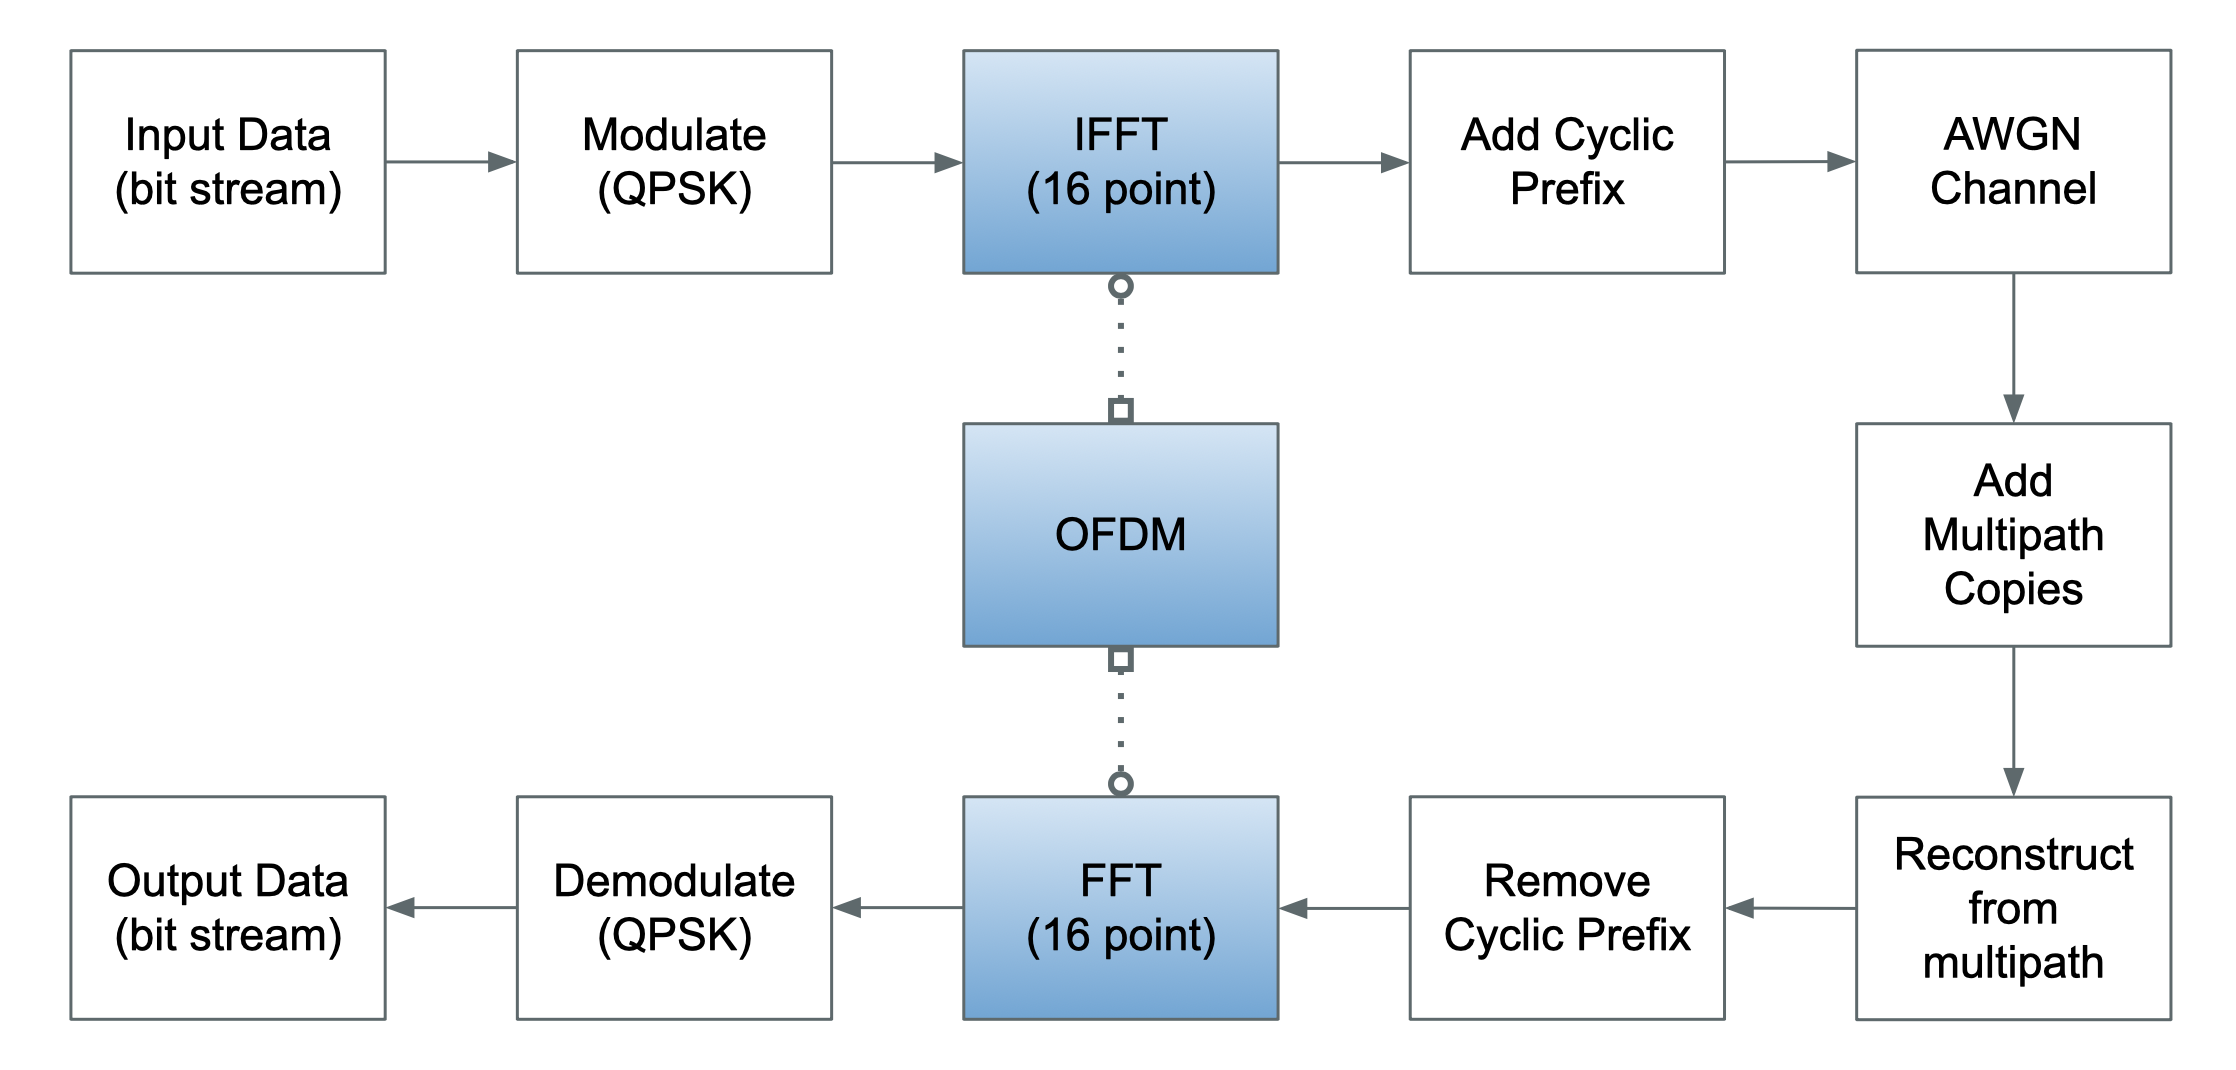
\includegraphics[width=0.5\textwidth]{./asset/OFDM_pipeline}
    \caption{OFDM pipeline}
    \label{fig:OFDM_pipeline}
\end{figure}
For OFDM part, Figure~\ref{fig:OFDM_pipeline} is our OFDM pipeline. The input data is bitstream. The colored box are unique for OFDM part.
    \hfill\\\subsubsection{QPSK}\hfill\\
    \indent We first do the modulation with QPSK ( Quadrature Phase Shift Keying ), this is just an extra modulation. Then we get the modulated data, or we can say the input data for OFDM.

    \hfill\\\subsubsection{OFDM}\hfill\\
    \indent The second part is the real OFDM modulation part, it is not complex at all. All we need is to apply the IFFT to our data and that’s it. OFDM is to map the data to orthogonal bases and IFFT is doing exactly the same thing. Each coefficients are on orthogonal basis which will not influence with each other.

    \hfill\\\subsubsection{Cyclic Prefix}\hfill\\
    \indent After that, we added the cyclic prefix for each symbol. The length of it is manually chosen to be larger than the multi-path delay.

    \hfill\\\subsubsection{Add White Gaussian Noise}\hfill\\
    \indent The third part is to add white gaussian noise to model the real transmission condition. The standard deviation of the noise will affect the final result of BER ( Bit Error Rate ) so we will change the standard deviation of the noise and average the result of BER so as to reduce the randomness.

    \hfill\\\subsubsection{Multi Path Fading}\hfill\\
    \indent The fourth part is to model the real channel, the white gaussian noise is not enough, we have to also add multi-path shading effect. We implemented it by copying the whole signal and add delay to it. With multiple copied version and the original version added together, we get the real signal in the ‘physical channel’.
\\\\
\textbf{The construction part of the OFDM pipeline ends here, following is the reconstruction part of the OFDM pipeline.}
    \hfill\\\subsubsection{Multi Path Fading reconstruction}\hfill\\
    \indent The first step is to remove the multi-path copies. In the real situation, we don’t know the delay time for each copy, we also don’t know the amplitude change for each copy, in our code, we just pass all these hyper-parameters from the transmission part to the reconstruction part. It’s too hard to learn about channel estimation and after all it’s not the core of our topic.
    % \hfill\\% \subsubsection{Add White Gaussian Noise reconstruction}\hfill\\

    \hfill\\\subsubsection{Cyclic Prefix reconstruction}\hfill\\
     \indent The second step is to remove the cyclic prefix. We already know the length of the cyclic prefix length, now that we already removed the multi-path effect, all we need to do is to delete cyclic prefix from the front of the symbol.

    \hfill\\\subsubsection{OFDM reconstruction}\hfill\\
    \indent The third step is to reconstruct from the OFDM. Now that we know for OFDM, what we do is just IFFT, so for reconstruction for OFDM, what we do is just FFT. After this part, we will get the signal before the OFDM.

    \hfill\\\subsubsection{QPSK reconstruction}\hfill\\
    \indent The fourth step is to reconstruct from the QPSK. There is already a function for us to use in Matlab so this part is also easy to implement. After the demodulation for QPSK, we can finally get the bit stream we sent into this OFDM system.

\subsection{FDM pipeline}
\begin{figure}[h]
    \centering
    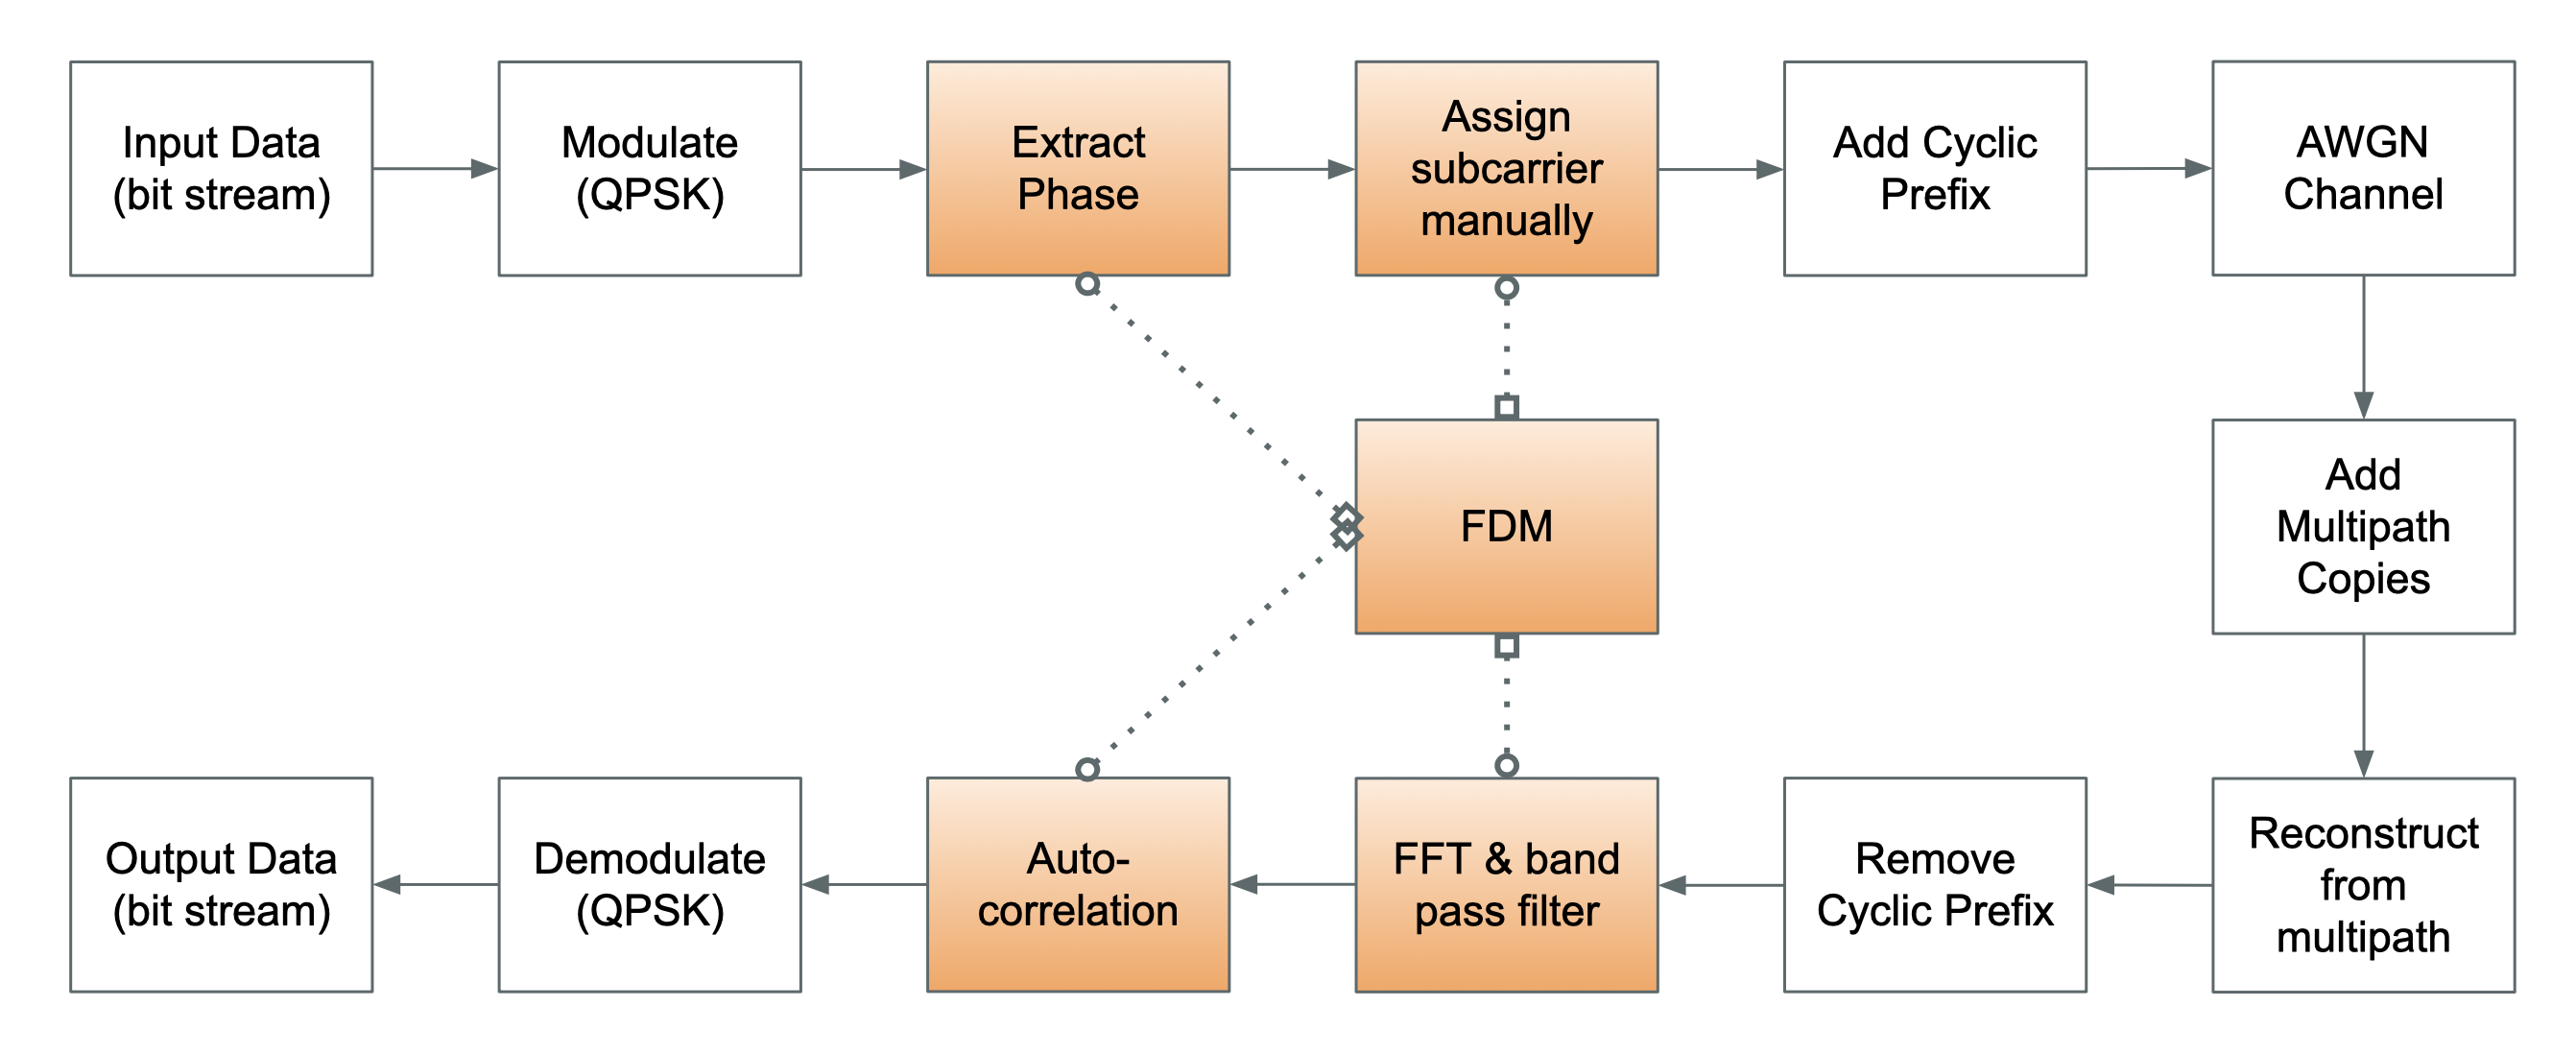
\includegraphics[width=0.5\textwidth]{./asset/FDM_pipeline}
    \caption{FDM pipeline}
    \label{fig:FDM_pipeline}
\end{figure}
For FDM part, Figure~\ref{fig:FDM_pipeline} is our FDM pipeline. The input data is bitstream. The colored box are unique for FDM part.

\hfill\\\subsubsection{QPSK}\hfill\\
    \indent The first step is still QPSK modulation. We want this step to be exactly the same as the OFDM pipeline. The reason why we want to use an extra modulation is because we want to compare different modulation method over here. But we didn’t have time to test all the other modulation schemes such as AM,FM.

    \hfill\\\subsubsection{FDM}\hfill\\
    \indent The second step is to do the FDM part. The FDM part is much more complicated than OFDM’s IFFT. For FDM part, we are facing three small steps. They are extracting the phase from the QPSK modulation, assign subcarriers manually.

    % \begin{itemize}
    %     \item \textbf{extract the phase}

    %     \item \textbf{assign subcarriers}
    % \end{itemize}
    \hfill\\\subsubsection{FDM: Extract the Phase}\hfill\\
    \indent The first small step for FDM is to extract the phase. After the QPSK, the bits turned into complex numbers. To feed them into the later FDM pipeline, we have to extract the phase manually. The reason why in the OFDM pipeline we don’t need to do that is because IFFT in OFDM can take in complex number while in our implementation of FDM, we can only take in the real phase information to insert in the cos function.

    \hfill\\\subsubsection{FDM: Assign Subcarriers}\hfill\\
    \indent The second small step for FDM is to assign subcarriers manually. After we get the phase from QPSK, we need to insert the phase into cos functions. One important thing that we need to justify is the baud rate. For OFDM, when using the IFFT, the signal length before and after the IFFT is the same. However, for FDM, now we have to put our signal on a carrier cos(fc*2*pi*t+phase), we have to lower the baud rate because we cannot represent this carrier just with one point. We have to at least have m points so as to first reconstruct the carrier frequency fc and then to extract the phase. How to choose this fc is a big problem, not to say how to tune the baud rate. What’s more, we have to also control the sampling frequency. This sampling frequency controls the gap of index variable t. We still don’t get a good conclusion about how to pick them. I think the reason about why the result of FDM part looks weird is mostly because of poor choice for variables fs and fc.


    \hfill\\\subsubsection{Multi Path Fading}\hfill\\
    \indent The third step for FDM is to add the cyclic prefix. This part is the same as the OFDM pipeline.
\\\\
\textbf{The construction part of the OFDM pipeline ends here, following is the reconstruction part of the OFDM pipeline.}
    \hfill\\\subsubsection{Multi Path Fading reconstruction}\hfill\\
    \indent The first and second step in FDM pipeline are the same of the OFDM pipeline. Just to remove the multi-path fading effect .

    \hfill\\\subsubsection{Cyclic Prefix reconstruction}\hfill\\
     \indent The first and second step in FDM pipeline are the same of the OFDM pipeline. Just to remove the cyclic prefix.

    \hfill\\\subsubsection{FFT}\hfill\\
    \indent The third step in FDM pipeline is to apply the FFT and band pass filter. This step is to separate the FDM bands manually. FFT can help us to transfer the time domain signal into frequency domain signal. After that, we can apply the band pass filter to pull out each FDM band we are using.

    \hfill\\\subsubsection{Extract Phase}\hfill\\
    \indent The fourth step in FDM pipeline is to extract the phase from the signal. The way we were using in this step is to do cross-correlation. We generate the template phase signal for each carrier frequency ( fc ), the template signal should be like cos( fc*2*pi*t + phase). After the cross-correlation, we would get the  phase for this carrier.


    \hfill\\\subsubsection{QPSK reconstruction}\hfill\\
    \indent The fifth step in FDM pipeline is to do the demodulation of QPSK. We have already extract the phase of the signal so all we need to do is to apply the inverse QPSK function to the phase. After this step, we would get the original bit stream.

\subsection{Result comparison}
The result we were using to compare the OFDM and FDM are BER ( bit error ratio ), throughput, ??? .

    \subsubsection{BER}\hfill\\
For the FDM BER, we didn’t get a good BER plot. The tricky thing is about choosing the fs ( sampling frequency ), fc ( carrier frequency ) and baud rate.
\begin{itemize}
    \item \textbf{fs}\\
 fs can influence the gap of time index t.  $\Delta t=\frac{1}{f_s}$.

    \item \textbf{fc}\\
fc can influence on which channel we are transmitting. Now that the fcs are chosen manually, to reduce aliasing between fcs, each fc should be more separate between each other. In our code, because we are setting the carrier frequency manually the fc to what we set. However, in the real live situation, the carrier frequency might be around the fc. That’s why if doing real life FDM simulation, we also need to calculate bandwidth of the carrier frequency and separate them with guard band. In our code, because it’s ideal, the carrier frequency bandwidth =0 and we don’t need guard band.

\item \textbf{baud rate}\\
The baud rate and the sampling frequency can determine the throughput. Using these two, we can calculate how much point we need to represent each carrier symbol. If the sampling frequency is 2000 1/sec and the baud rate is 500 bits/sec, then each carrier symbol will need 4 time index to represent.
\end{itemize}
To get the BER for FDM, we tried different combinations of these three hyper-parameters. However, the result we get isn't so well.

We also compared two versions of OFDM. One is with the multi-path fading effect, the other one is without multi-path fading effect. This comparison is just to see if the cyclic prefix does work. From the figure, we can see that especially when the SNR ( signal to noise ratio ) is really high, the cyclic prefix did improve the BER a lot.


\section{Hardware Simulation}



% \begin{figure}[h]
%     % test figure
%     \centering
%     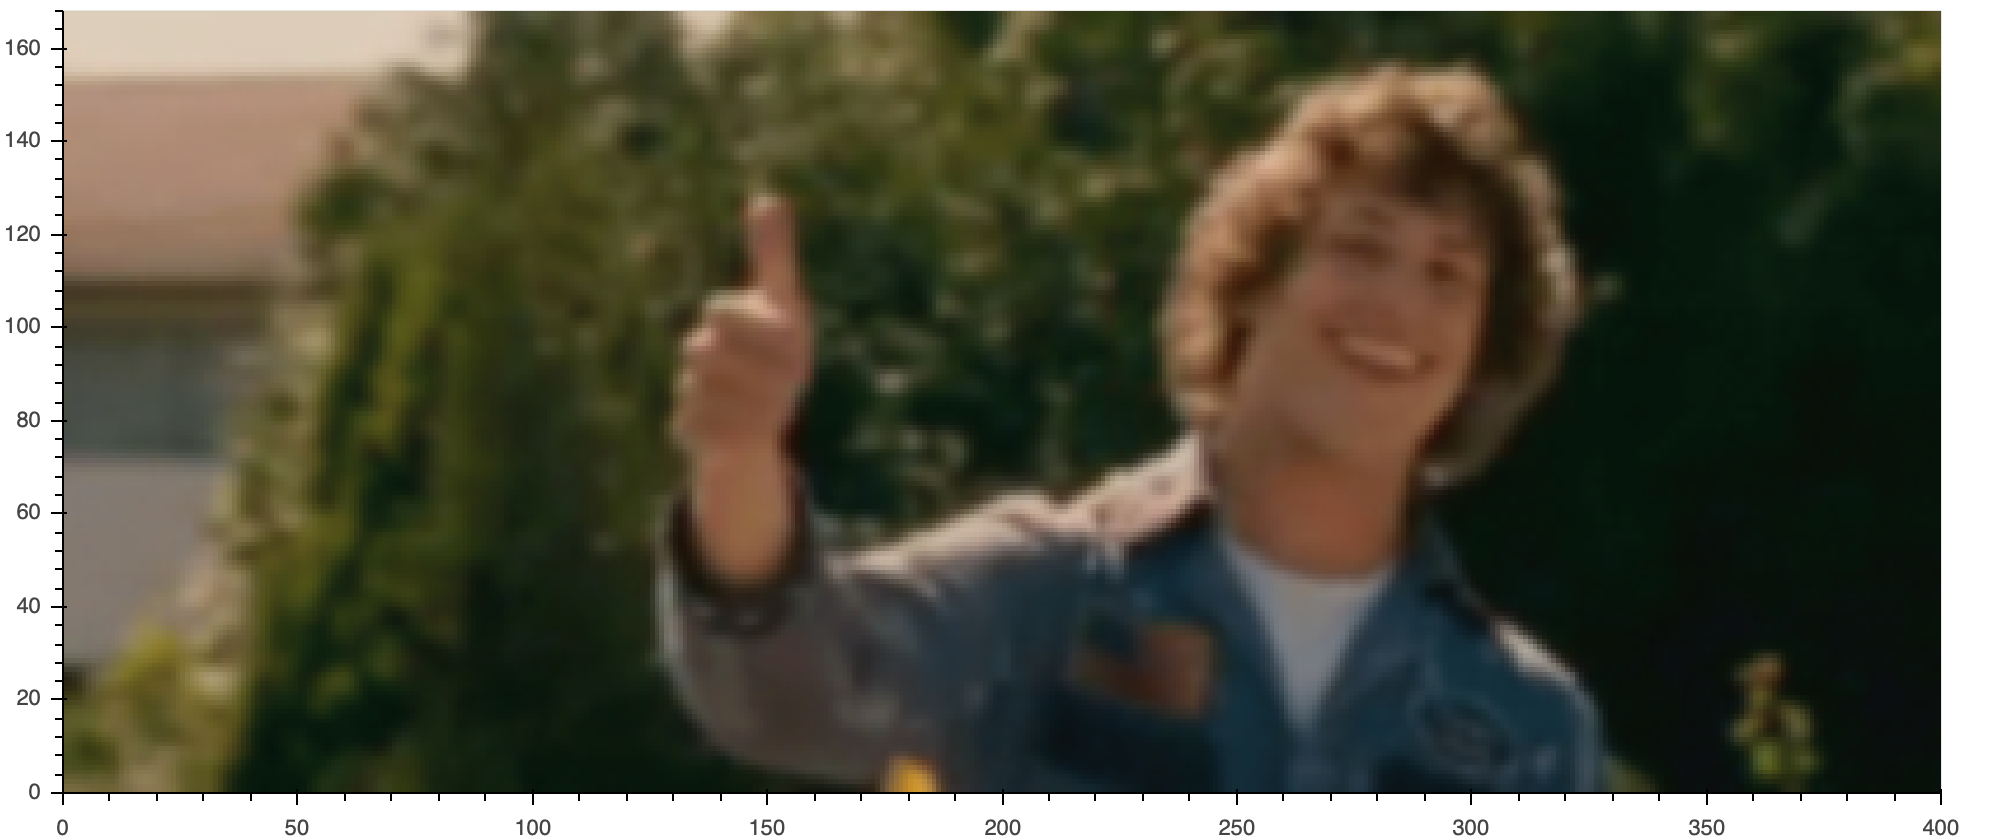
\includegraphics[width=0.5\textwidth]{./asset/test.png}
%     % \caption{Figure P2_63-1}
%     % \label{fig:2_63}
% \end{figure}

%     %test formula
%     \[\begin{aligned}
%         y[n]&=(x[n]\cdot e^{-j\omega_0n})*h[n]\\
%         &=\sum_{m=-\infty}^{\infty}x[n-m]\cdot e^{-j\omega_0(n-m)}\cdot h[m]\\
%         if\quad x[n]&=a x_1[n]+bx_2[n]\\
%         y[n]&=\sum_{m=-\infty}^{\infty}(a x_1[n-m]+bx_2[n-m])\cdot e^{-j\omega_0(n-m)}\cdot h[m]\\
%         &=a\times \sum_{m=-\infty}^{\infty}x_1[n-m]\cdot e^{-j\omega_0(n-m)}\cdot h[m]+b\times \sum_{m=-\infty}^{\infty}x_2[n-m]\cdot e^{-j\omega_0(n-m)}\cdot h[m]\\
%         &=ay_1[n]+by_2[n]
%     \end{aligned}\]


%     % test bracks
%     \[\begin{cases}
%         \quad \mathcal F \{x[n]\}&=X(\omega)\\
%         \quad \mathcal F \{h_i[n]\}&=H(\omega)
%         \end{cases}\]
%     % test
%     \begin{enumerate}
% 	\item \textbf{What is the impulse response of the system?}\\
% 	\item \textbf{Is the system causal?}\\
%   	 I think the system is not casual because the transfer function has infinit support. When doing convolution, we have to know the value in the future.
%   	\item \textbf{Is the system BIBO stable?}\\
% 	\end{enumerate}


\end{document}